\documentclass[a0paper,landscape]{xebaposter}

\usepackage{qrcode}
\usepackage[intlimits]{amsmath} 
\usepackage{graphicx,xcolor, xecolor}
\graphicspath{{images/}}
\usepackage{listings}
\usepackage[inline]{enumitem}
\setlist{noitemsep}
\usepackage{wrapfig}
\usetikzlibrary{shadows,calc,shapes.callouts, positioning}

\usepackage{xepersian}
\settextfont[Scale=1]{XB Niloofar}
\setlatintextfont[Scale=.9]{Linux Libertine}
\setdigitfont{Yas}
\defpersianfont\Yas{Yas}

\defpersianfont\adobe[Scale=1.2]{Adobe Arabic}
\setsayehfont[Scale=1.3]{XB Kayhan Navaar}
\setiranicfont [Scale=1.4]{XB Zar}%Oblique}
\defpersianfont\Navar[Scale=1.6]{XB Kayhan Navaar}

\background{
\begin{tikzpicture}[remember picture, overlay]
\node [rotate=45, opacity=.3,  scale=8] at (current page.center)  
        {$\displaystyle F(u)=\int_{-\infty}^{+\infty}f(x)e^{-\pi i ux} \mathrm{d}x$};
\end{tikzpicture}
}

\begin{document}
\begin{poster}
    {columns=3,
      headershape=rounded, 
      headerborder=closed, 
      borderColor=gray, 
      headerheight=.08\textheight,
      background=user, }
    {
\includegraphics[height=.08\textheight]{qomlogo.png}}
    {\Navar مجموعهٔ پارسی لاتک ۱۳۹۵}
    {}
        {
\includegraphics[height=.08\textheight]{parsilatexlogo.png}}

\begin{posterbox}[name=doyouknow, column=1]{آیا می‌دانید؟!}
\begin{description}
\item[آیا]
 می‌دانید  که در بسیاری از دانشگاههای معروف دنیا مانند استنفورد و برکلی از نرم‌افزاری به غیر از \lr{Microsoft Word} برای نگارش مستندات علمی استفاده می‌شود؟
\item[آیا]
 از تنظیم حاشیه، تغییر قلم و به طور کلی انجام صفحه‌آرایی مستندات خود خسته شده‌اید؟

\item[آیا]
 علاقمند هستید انجام صفحه‌آرایی نوشته‌هایتان را به یک صفحه‌آرای حرفه‌ای بسپارید؟
\item[آیا]
 می‌دانید در صورت استفاده از سیستم حروف‌چینی تِک/لاتِک امکانات گسترده‌ای برای آماده‌سازی مستندات علمی دارید؟ امکاناتی همچون:
\begin{itemize}
\item  مدیریت راحت مراجع
\item  تایپ دستی فرمولها، بدون نیاز به ماوس
\item  کلاسهای آماده برای تایپ مقاله و پایان‌نامه
\item  درج الگوریتم‌ها و برنامه‌های شکیل و یکسان
\item  رسم نمودارها و اشکال بسیار متنوع و با کیفیت بالا
\item  درج جداول و نمودارهای تولید شده  با برنامه‌ای همچون \lr{MATLAB} مستقیماً در فایل مقاله یا پایان‌نامه شما
\end{itemize}

\end{description}
\end{posterbox}

\begin{posterbox}[name=samples, below=doyouknow, column=1]{نمونه سند و مثال از لاتک}
%\centerline{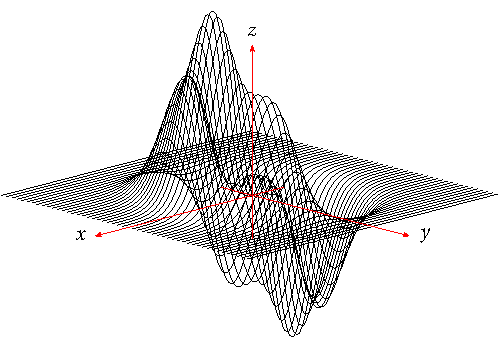
\includegraphics{plot.pdf}}

\makeatletter\lstset{% general command to set parameter(s)
    basicstyle=\setLTR\@nonlatinfalse\footnotesize\ttfamily,
    captiondirection=RTL, captionscript=nonlatin, 
    language=[LaTeX]tex,    numbers=left, numberstyle=\tiny\Yas, numbersep=4pt, 
    frame=l,%    frameround=L,    
    gobble=0,    breaklines=true,    escapechar={|},
    aboveskip=2\medskipamount,
}
\begin{tikzpicture}[auto,bend right, rounded corners=2pt, inner sep=1.4pt, ]
\node (latinsample) [draw, fill=white,
    general shadow={shadow xshift=-3pt, shadow yshift=-3pt, fill=gray} ,  ]
 {
\hspace{3mm}\begin{minipage}{.65\linewidth}
\begin{lstlisting}
\documentclass{article}
\begin{document}
Hello world!
\end{document}
\end{lstlisting}
\end{minipage}};
\node [ color=white, fill=gray, draw, ]at (latinsample.north) {\Yas\rl{یک مثال ساده با لاتک }};

\node (persiansample) [anchor=north, general shadow={shadow xshift=-3pt, shadow yshift=-3pt, fill=gray} ,
     fill=white, xshift=-.6cm, yshift=.75cm,]
    at (latinsample.south east) {
\hspace{3mm}\begin{minipage}{.65\linewidth}
\begin{lstlisting}
\documentclass{article}
\usepackage{xepersian}
\settextfont{Yas}
\begin{document}
|\hfill\beginR\rl{سلام.} \rl{به دنیای} \textbackslash{}LaTeX \rl{خوش آمدید.}\endR|
|\hfill\rl{با کمک بسته‌ٔ زی‌پرشین می‌توانید از بسیاری از قابلیت‌های  }|
|\hfill\rl{لاتک همچون فرمول‌نویسی، مانند }|
$\sum_{i=1}^n i=\frac{n(n+1)}{2}$ 
|\hfill\rl{در زبان فارسی استفاده کنید.}|
\end{document}
\end{lstlisting}
\end{minipage}};
\node [ color=white, fill=gray, draw, ]at (persiansample.north) {\Yas\rl{یک مثال ساده با بستهٔ زی‌پرشین }};
\node (plot) at (persiansample.south) [opacity=.5, anchor=north, yshift=-1cm] 
        {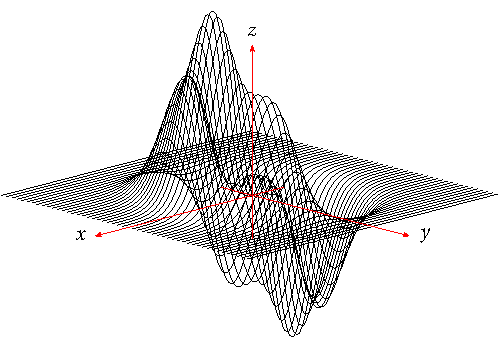
\includegraphics{plot.pdf}};
\node (func) at (persiansample.south) [color=white, fill=black!90, 
            rectangle callout, draw,  callout pointer shorten=2cm,
            callout absolute pointer={ ($(plot.center)$), },
%            above left= 5pt and 0pt of plot.north east,
%            callout relative pointer={(-2, -3)}, %callout pointer width=.5cm,
%            callout pointer anchor=south east,
%            ,anchor=north, 
            yshift=-.5cm, xshift=-2.5cm] {
$z(x,y)=10\left(x^3+xy^4-\frac{x}{5}\right)e^{-(x^2+y^2)}+e^{-\left((x-1.225)^2+y^2\right)}$
};
%\draw  [->, very thick] ($(func.south west)+(1.2cm,0)$) to ($(plot.center)-(3.5cm,.5cm)$);
%\node [starburst, draw,starburst points=72, anchor=center] at (current bounding box.south) {
%\centerline{\rl{\adobe این پوستر تماماً تحت سیستم حروف‌چینی \lr{\LaTeX} با استفاده از بسته \lr{\XePersian}}} \\
%\centerline{\rl{\adobe و طبقهٔ نوشتاری {\ttfamily xebaposter} آماده شده است.}}};
\end{tikzpicture}

\vspace{-5mm}
\begin{quote}\centering
{\adobe این پوستر تماماً تحت سیستم حروف‌چینی
 \lr{\LaTeX} با استفاده از بسته \lr{\XePersian} 
 و طبقهٔ نوشتاری {\ttfamily xebaposter} آماده شده است.}
 \end{quote}
\end{posterbox}
%\end{poster}\end{document}

\begin{posterbox}[name=tex, column=2]{تک/لاتک  (\lr{\TeX/\LaTeX})}
\adobe
\begin{wrapfigure}{r}{4cm}

\includegraphics[width=0.4\columnwidth]{lion.png}
\end{wrapfigure}


تِک (\TeX) نرم‌افزاری مخصوص حروف‌چینی است که در سال ۱۹۷۸ توسط پروفسور دونالد کِنوث، استاد دانشگاه استنفورد به دنیا معرفی شد. به دلیل کیفیت حرفه‌ای مستندات تولید شده توسط آن، وجود مجموعه ابزار بسیار متنوع برای حروف‌چینی مستندات در رشته‌های مختلف همچون ریاضی، کامپیوتر و فیزیک، تِک تبدیل به نرم‌افزار مورد استفاده بسیاری از ناشران شده است.

    تک با همهٔ مزایایی که دارد، برای استفاده گسترده و کاربر پسند دارای یک مشکل اساسی است: تک یک زبان برنامه نویسی واقعی، 
    گسترده و مشکل
    است که یادگیری و به کارگرفتن آن برای کاربران عادی پرزحمت و غیراقتصادی است. لاتک (\lr{\LaTeX{}})
     که در سال $1984$ توسط پروفسور لزلی لمپورت 
     به وجود آمد، در واقع تکمیل تک بود؛ با همهٔ چیزهایی که لازم بود به آن اضافه شود تا به
    محصولی قابل استفاده برای عموم تبدیل گردد. تعداد زیادی امکانات امنیتی و پیغام‌های خطا، همچنین قالب‌های مختلف متن
    (کتاب، نامه، گزارش و...)، امکانات فراوان برای ایجاد فصل‌ها، بخش‌ها، فهرست مطالب، فهرست نمایه، 
    فهرست منابع و ایجاد پیوندهای مورد نیاز برای ساختن این فهرست‌ها در متن سند،
    از جمله امکاناتی هستند که در کنار سیستم حروفچینی و صفحه بندی تک، لا‌تک را به وجود می‌آورند.

    از زمان ارائهٔ لا‌تک، استفاده از آن، به شیوهٔ اصلی بهره‌گیری از سیستم تک برای تولید اسناد تبدیل شده است. اهمّیت تک به عنوان قلب
    اصلی سیستم، همچنان محفوظ است، امّا کاربران عموماً با لا‌تک کار می‌کنند. تک و لا‌تک هر دو با مجوزهای نرم افزار آزاد منتشر شده‌اند
    و کد منبع آن‌ها در دسترس همگان قرار دارد.
\end{posterbox}

\begin{posterbox}[name=xepresian, column=2, below=tex, ]{زی‌پرشین  (\lr{\XePersian})}
\adobe
\begin{wrapfigure}{l}{4cm}

\includegraphics[scale=.3]{xepersian-logo.pdf}
\end{wrapfigure}

    زی‌پرشین یک بسته مخصوص لاتک است که با همت آقای وفا خلیقی  آماده شده و با استفاده از آن می‌توانید از بسیاری 
    از قابلیت‌های سیستم تک/لاتک برای حروف‌چینی مستندات فارسی خود استفاده کنید. 

    در زی‌پرشین بسیاری از امکانات لاتک به گونه‌ای تغییر داده شده است تا برای زبان فارسی نیز قابل استفاده باشد.
    همچنین زی‌پرشین با اضافه کردن برخی از ویژگی‌های زبان فارسی مانند کشیدگی حروف،
    حروفچینی را برای کاربران فارسی زبان ساده‌تر نموده است. از دیگر ویژگی‌های زی‌پرشین می توان به امکان حروفچینی
    دوجهته و انواع شماره‌گذاری‌ها اشاره نمود. در ذیل به برخی از دیگر ویژگی‌های این بسته اشاره شده است:

    \begin{enumerate*}[label=\Yas\arabic*)]
        \item    پشتیبانی از ورودی با رمزینهٔ یونیکد؛
        \item    استفادهٔ مستقیم از تمامی قلم‌های نصب‌شده بر روی سیستم عامل؛ \pagebreak
        \item    تولید خروجی با قالب \lr{PDF}؛
        \item  {  توانایی استفاده از ویژگی‌های خاص \lr{PDF} که آن را برای تولید مستندات الکترونیکی و
                    نیز ارائهٔ الکترونیکی، علاوه بر مستندات چاپی، مناسب می‌کند (مثلاً اسلایدسازی از ویژگی‌های خاص \lr{PDF}
                    استفاده می‌کند و این بسته در زی‌پرشین قابل استفاده است)}؛%\pagebreak
        \item    قابل جستجو بودن \lr{PDF} تولید شده،
        \item    پشتیبانی از نسخه جاری و فعال لاتک (\lr{\LaTeXe})؛
        \item    قابل اجرا بر روی اکثر سیستم عامل‌های موجود (مانند ویندوز، لینوکس، و مک)؛
        \item    عدم نیاز یا وابستگی به ویرایشگر (یا نرم‌افزار) مخصوص برای تهیه فایل ورودی؛
        \item    عدم نیاز به یادگیری دستورات جدید در صورتی که با دستورات لاتک آشنایی قبلی داشته باشید؛
        \item    حجم بسیار کم کل بسته (در صورت وجود یک توزیع تک که موتوز زی‌تک را داشته باشد) و
        \item    موجود بودن بسته در مخزن دو توزیع عمده تک که عبارت از
            \lr{MiK\TeX} و \lr{\TeX{}Live} هستند.
    \end{enumerate*}

به‌علاوه با همکاری جمعی از دانشجویان و اساتید داخل و خارج از کشور امکانات دیگری همچون ویرایشگر دوجهته، مبدل فارسی‌تک به زی‌پرشین، سایت و تالار پرسش و پاسخ در خصوص استفاده از زی‌پرشین ، نمونه مثال‌ها و  بستهٔ قابل نصب نیز فراهم شده است.

%\begin{itemize}
%	\item شکل رسم شده متعلق است به تابع 
%	$z(x,y)=10\left(x^3+xy^4-\frac{x}{5}\right)e^{-(x^2+y^2)}+e^{-\left((x-1.225)^2+y^2\right)}$.
%	\item  برای آشنایی بیشتر با فارسی نویسی در لاتک می‌توانید به تارنمای \url{http://www.
%tex.com} مراجعه نمایید. 
%	\item \textxecolor{green}{\myText}
%\end{itemize}

%%{\scriptsize $z(x,y)=10\left(x^3+xy^4-\frac{x}{5}\right)e^{-(x^2+y^2)}+e^{-\left((x-1.225)^2+y^2\right)}$}
\end{posterbox}

\begin{posterbox}[name=parsilatex, column=0]{مجموعهٔ پارسی لاتک}

\centerline{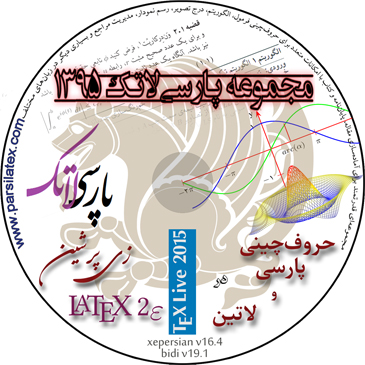
\includegraphics[scale=3]{parsilatexdvd.png}}

مجموعه پارسی‌لاتک شامل ابزارهای لازم برای حروف‌چینی با سیستم لاتک و بسته زی‌پرشین است که با دقت و وسواس فراوانی توسط گروه پارسی‌لاتک آماده شده است. 
%کلیه نرم‌افزارهای موجود در این مجموعه، رایگان بوده و از طریق اینترنت پرسرعت قابل دانلود است. 
%با این حال برای رفاه حال کاربرانی که به اینترنت پرسرعت دسترسی ندارند، امکان خرید پستی این مجموعه فراهم شده است.

محتویات این دی‌وی‌دی به شرح زیر است:
\begin{itemize}
    \item 
توزیع تک‌لایو $2015$ برای نصب روی سیستم‌عامل‌های ویندوز و لینوکس با راهنمای نصب فارسی
    \item 
راهنمای استفاده از بسته‌های تک‌لایو از جمله راهنمای بسته‌های زی‌پرشین و بی‌دی
    \item 
مجموعه‌فیلم‌های آموزش لاتک دکتر فرشاد ترابی
    \item 
فایل‌های صوتی معرفی بسته زی‌پرشین آقای امیرمسعود پورموسی
    \item 
چندین نمونه‌‌مثال‌ زی‌پرشین جهت حروف‌چینی مقاله، پروپوزال، سمینار، پایان‌نامه، رساله و…
    \item 
ویرایشگرهای موردنیاز مانند تک‌میکر، تک‌ورکس و تک‌استودیو برای نوشتن و ویرایش فایل‌های تک
    \item 
فونت‌های فارسی استفاده شده در مثال‌های داخل دی‌وی‌دی
    \item 
چند نرم‌افزار کاربردی مانند نرم‌افزار طراحی شکل و نمودار، مفسر زبان پرل و پایتون، کیبورد استاندارد فارسی برای سیستم‌عامل ویندوز، ویرایشگر متنی \lr{gedit} و \lr{gvim}
\end{itemize}

\end{posterbox}

\begin{posterbox}[name=parsilatex, column=0, below=parsilatex]{دی‌وی‌دی مجموعهٔ پارسی‌لاتک را از کجا تهیه کنیم؟}

 
\begin{minipage}{.2\linewidth}
    \qrcode[height=.8in]{http://parsilatex.com/site/?p=185}
\end{minipage} 
\hfill
\begin{minipage}{.78\linewidth}
    این دی‌وی‌دی توسط گروه پارسی‌لاتک عرضه می‌گردد که می‌توانید آن را به صورت آنلاین از طریق سایت گروه پارسی‌لاتک 
    به قیمت $18500$ تومان سفارش دهید. 
    
    طی هماهنگی انجام شده بین دانشکده علوم‌پایه و آن گروه، 
    می‌توانید این دی‌وی‌دی را با $40$\% تخفیف به قیمت $11000$ تومان ابتیاع نمایید.     
    برای تهیه دی‌وی‌دی به آقای صفری در دانشکده علوم‌پایه مراجعه فرمایید.
\end{minipage}
\end{posterbox}

\end{poster}
\end{document}
